%-----------------------------------------------------------------------------%
\chapter{\babDua}
\label{bab:2}
%-----------------------------------------------------------------------------%
\todo{
	Bab ini, biasanya namanya adalah "Studi Literatur" atau "Tinjauan Pustaka".
	Akan tetapi, beberapa fakultas atau dosen pembimbing meminta Bab 2 untuk dinamakan lain, seperti "Kerangka Berpikir".
}

Untuk memulai penelitian, dibutuhkan kerangka berpikir yang sesuai untuk permasalahan yang ingin dipecahkan.
Untuk membentuk kerangka berpikir yang sesuai, perlu dikaitkan dengan hasil studi literatur yang telah dilakukan.
Oleh karena itu, pada bab ini, akan dijelaskan hasil studi literatur yang telah dilakukan yang telah dikaitan dengan kerangka kerja untuk penelitian ini.

This chapter


%-----------------------------------------------------------------------------%
\section{Related Works}
\label{sec:Related Works}
%-----------------------------------------------------------------------------%
\subsection{Lattice-Based Cryptography}
A lattice is a discrete subset of n-dimensional vectors of real numbers $\mathbb{R}^n$ formed by all integer linear combinations of a set of linearly independent basis vectors. Formally, given a basis $\mathbf{B} = \{ \mathbf{b}_1, \dots, \mathbf{b}_k \} \subset \mathbb{R}^n$, a lattice $\mathcal{L}$ is defined as:
\[
\mathcal{L} = \left\{ \sum_{i=1}^{k} z_i \mathbf{b}_i \;\middle|\; z_i \in \mathbb{Z} \right\}
\]
Lattices can be visualized as regularly spaced grids extending in multiple dimensions, but their structure becomes increasingly complex and difficult to visualize in high-dimensional spaces, and especially beyond the third dimension.

Lattice-based cryptography relies on the presumed hardness of certain computational problems defined over lattices. Two of the most important problems are the Shortest Vector Problem (SVP), which asks for the shortest non-zero vector in a lattice, and the Learning With Errors (LWE) problem, which involves solving systems of linear equations that have small random noise. As of now, no algorithms exist that can solve these problems efficiently even with quantum computers, and they are tentatively believed to be quantum resistant.

Practical lattice-based schemes often use structured variants such as Ring-LWE and Module-LWE (MLWE), which operate over polynomial rings. These variants significantly improve efficiency while retaining the core hardness properties. MLWE in particular provides a balance between performance and conservative security assumptions and forms the basis of several standardized post-quantum schemes, including ML-KEM and ML-DSA. 

It should be noted that both ML-KEM and ML-DSA employ Number Theoretic Transform (NTT), a generalization of Discrete Fourier Transform (DFT) to finite fields, to accelerate polynomial multiplication. The NTT representation of a polynomial will be in hat notation(e.g., $\hat{A}$).

\subsection{Learning with Errors}
\mbox{}
Learning with Errors is essential for modern lattice-based post-quantum criptographic algorithms, such as NIST's ML-KEM and ML-DSA \cite{11}. Basically, this is a method to hide information (e.g plaintext) by injecting randomized noise (errors) into a system of linear equations which represents the public matrix, which would make the attackers struggle to get the actual pieces of the information from the plaintext. Solving an LWE problem means solving a set of linear equations with errors hidden in the equations. The errors are often tiny. 

For example, given the public matrix $A$, a secret message or plaintext $s$, and a random small number to mess the equation $e$. Normally, without the latter, a cipher is usually defined as $C = As \pmod q$. With LWE however, the equation becomes $C = As + e \pmod q$. Without the small errors, the system of linear equations can be solved with Gaussian Elimination, making it easier to crack. 

There are two types of LWE: 
\begin{itemize}
\raggedright
\item Search LWE: This approach is to find $s$, the secret key from a noisy set of linear equations. 

\item Decision LWE: This approach is to distinguish an equation with LWE from a pure random noise. Usually, a real LWE set of equations would actually at first look random, but the errors gained from the solutions (lattice reduction algorithms) of these equations do usually cluster around the actual key. 
\end{itemize}

The noise should be small enough that legitimate users can still recover the intended message. At the same time, the presence of this error prevents an attacker from directly solving the underlying system of linear equations using standard techniques such as Gaussian elimination. The best known attacks typically involve constructing a lattice from the problem instance and applying lattice reduction algorithms to search for unusually short vectors, thereby reducing the attack to problems closely related to SVP (Shortest Vector Problem). 

SVP itself is the problem of finding the shortest non-zero vector in a lattice \cite{12}. For a vector in a lattice to be regarded as the SVP, a vector must be the shortest one (or one of the shortest ones), out of all vectors in the lattice, and it must be a nonzero vector. It is essential for PQC lattice reduction algorithms because it can help to solve the LWE problem used in PQC algorithms. 

\subsection{ML-KEM - FIPS 203}
ML-KEM, also referred to as Module-Lattice-Based Key-Encapsulation Mechanism Standard, is a standard set by NIST’s FIPS 203 publication that specifies a set of algorithms meant to be used to establish a shared private key between two parties. This standard was proposed in response to the potential unreliability of modern cryptographic key systems such as RSA in the face of quantum computers.

ML-KEM is a variant of the CRYSTALS-Kyber algorithm \cite{2021kyber}, which is itself based on the hardness of solving MLWE, which is based on the presumed hardness of specific computational problems in module lattices. It can be described as a generalization of the Learning with Errors (LWE) problem as previously described. Both LWE and MLWE are widely considered to be quantum resistant, in that there are no known quantum algorithms that can solve them efficiently.

ML-KEM and other KEMs (Key Encapsulation Mechanisms) typically consist of three main algorithms: a key generation, key encapsulation, and key decapsulation algorithm.

\begin{figure}[H]
	\centering
	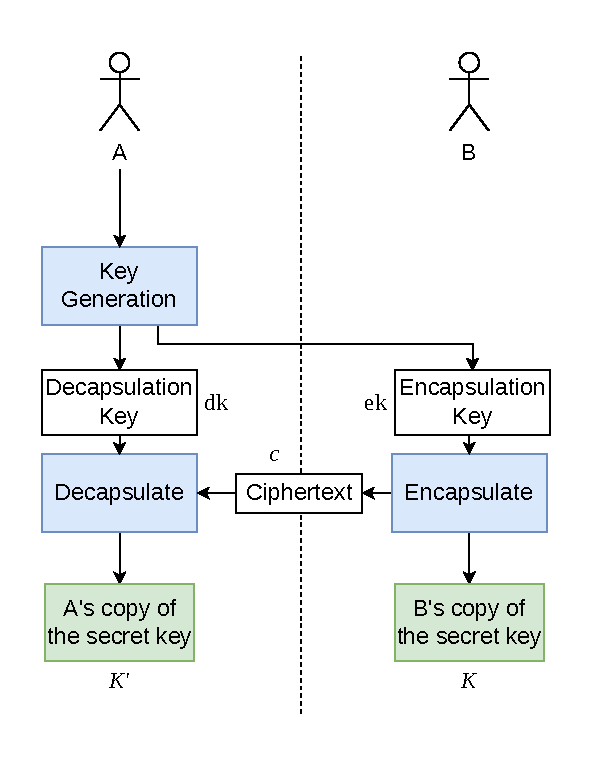
\includegraphics[width=.42\linewidth]{assets/pdfs/KEM_diagram.pdf}
	\caption{Simplified key establishment process using KEM}
	\label{fig1}
\end{figure}

As shown in Figure~\ref{fig1}, KEMs are used to establish a shared private key between two parties. Party A begins by running a key generation algorithm that produces an encapsulation (public) key and decapsulation (private) key. When party B accepts the encapsulation key, they can run the encapsulation algorithm with it as an input, which produces a copy of the two parties’ shared secret key \textit{K} and its associated ciphertext \textit{c}. Party B sends the ciphertext to party A, and party A runs the decapsulation algorithm using the decapsulation key and the ciphertext, producing their own copy \textit{K'} of the shared secret key.

They also have multiple parameter sets, of which ML-KEM has three. Each set specifies the underlying ring dimension, module rank, noise distributions, and compression parameters. Increasing these parameters results in larger matrices, vectors, and noise levels, which enhances security at the cost of computational efficiency. In order of least to most secure and most to least efficient, they are ML-KEM-512, ML-KEM-768, and ML-KEM-1024.

\begin{figure}[H]
	\centering
	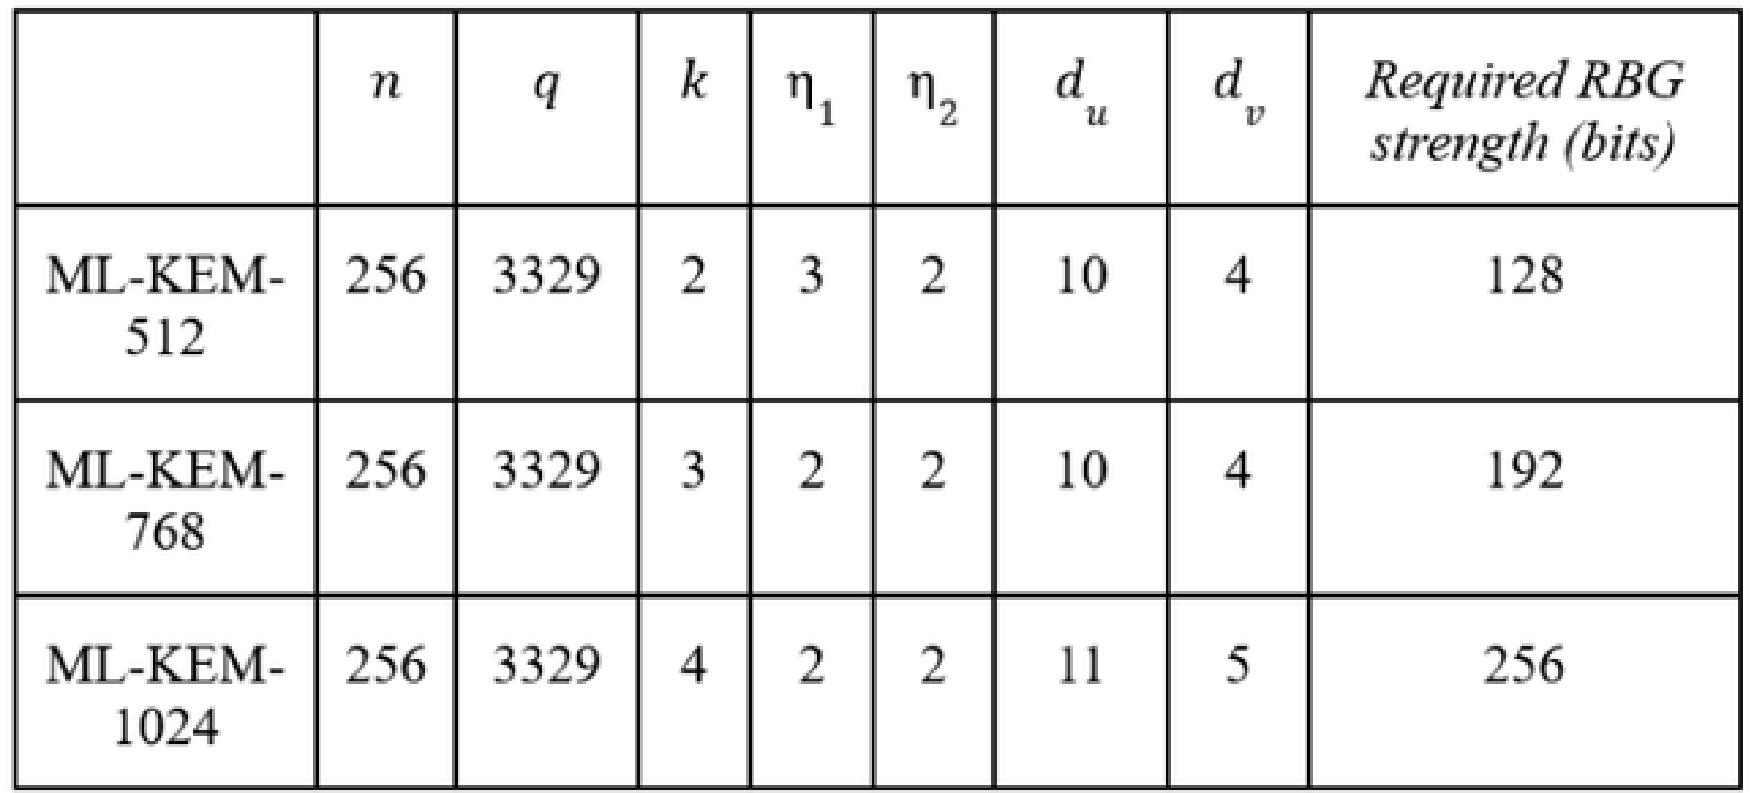
\includegraphics[width=.42\linewidth]{assets/pdfs/paramset_mlkem.pdf}
	\captionsource
        {Parameter sets for ML-KEM (Kyber) security levels}
        {\cite{nistfips203}}
	\label{fig:parameterkem}
\end{figure}

Each parameter set is comprised of the five individual parameters $k$, $\eta_1$, $\eta_2$, $d_u$, and $d_v$, and two constants $n$ and $q$.
\begin{itemize}
\item $k$ determines the dimensions of several matrices and vectors used throughout the algorithm and is the primary factor affecting the security level. An increase in $k$ comes with an increase in security level, key sizes, and ciphertext sizes, but also computational cost.
\item $\eta_1$ and $\eta_2$ specify the distributions used to generate the random noise terms that are fundamental to the security of the scheme; vectors $s$ and $e$ in K-PKE.KeyGen and the vector $y$ in K-PKE.Encrypt respectively. Essentially, increasing them produces larger noise terms and increases security level at the cost of efficiency.
\item $d_u$ and $d_v$ determine the level of compression applied to data during key encapsulation and are used by several encoding, decoding, compression, and decompression operations.
\item Constants $n$ and $q$ are the same between the three approved parameter sets. $n$ specifies the degree of the polynomial ring for the scheme, while $q$ is the modulus used for modular arithmetic.
\end{itemize}

\subsubsection{ML-KEM Key Generation}
The key generation algorithm ML-KEM.Keygen in ML-KEM produces an encapsulation key and decapsulation key using internally generated 32 byte seeds $d$ and $z$. These keys are used in the encapsulation and decapsulation algorithms to establish a secure shared secret over a potentially insecure communication channel.

\begin{figure}[H]
	\centering
	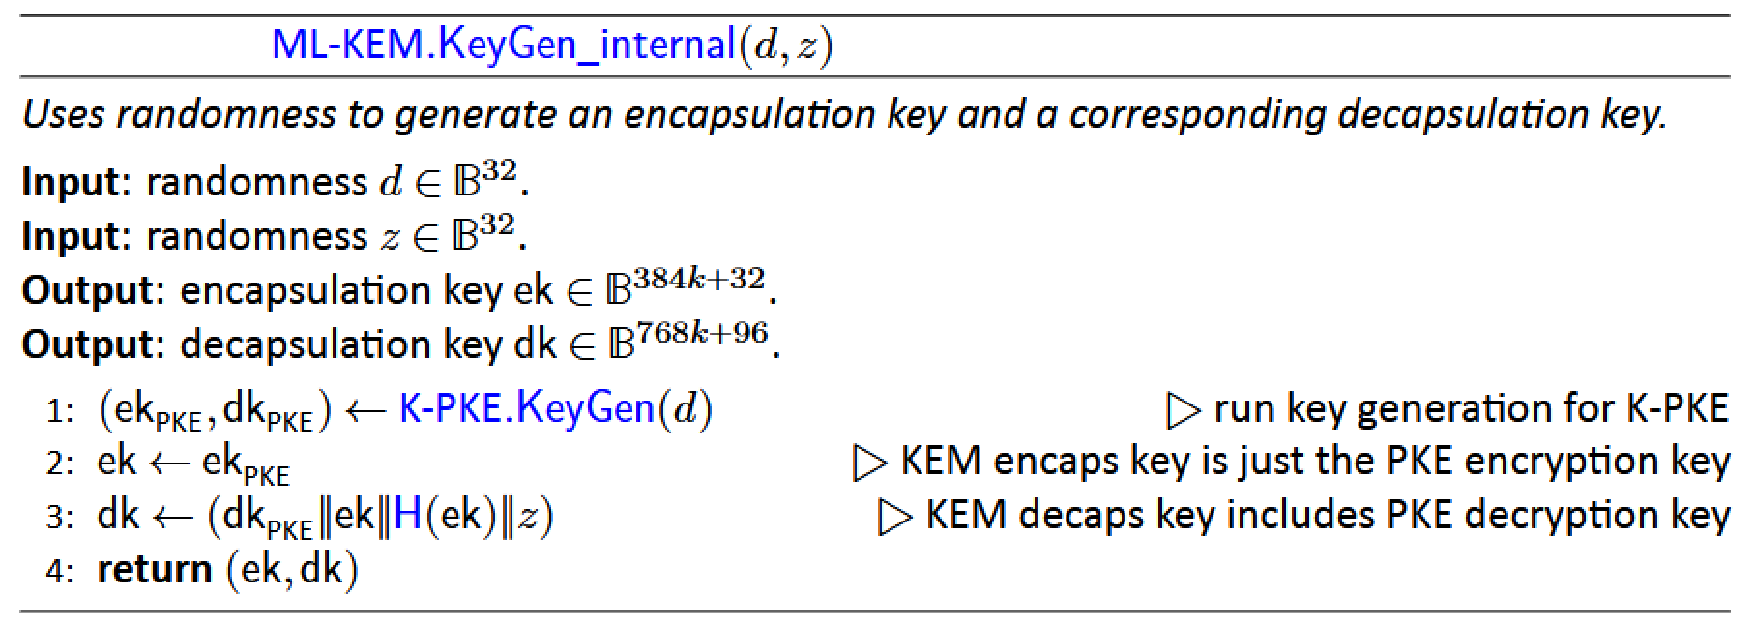
\includegraphics[width=.9\textwidth]{assets/pdfs/mlkem_keygen_internal_edit.pdf}
	\captionsource
		{ML-KEM.KeyGen() algorithm}
		{\cite{nistfips203}}
	\label{fig:mlkem-keygen-int}
\end{figure}

Assuming the generated random seeds $d$ and $z$ are valid, the seed $d$ is used to run Kyber’s key generation algorithm K-PKE.KeyGen, which outputs the encryption key and decryption key. The encryption key becomes the encapsulation key used by ML-KEM. The decapsulation key is constructed from the decryption key together with the encapsulation key, a hash of the encapsulation key, and the 32-byte random seed $z$.

\begin{figure}[H]
	\centering
	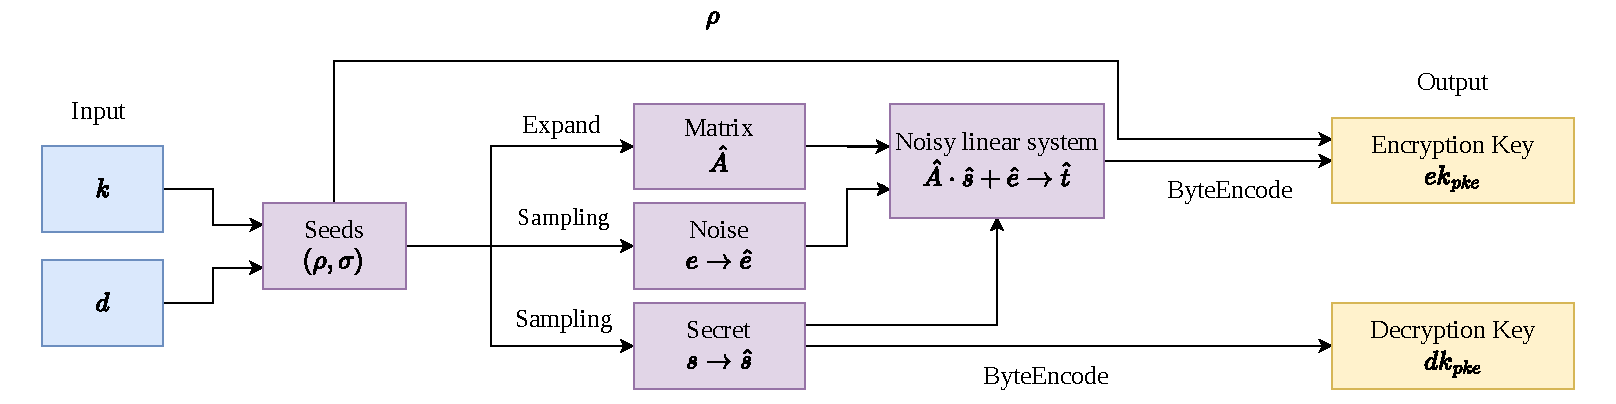
\includegraphics[width=1.0\linewidth]{assets/pdfs/kyber-keygen.pdf}
	\caption{Kyber Key Generation Algorithm K-PKE.KeyGen}
	\label{fig2}
\end{figure}

K-PKE.KeyGen begins by generating 32 byte seeds $\rho$ and $\sigma$ from hashing the input $d$ and $k$ from the chosen parameter set. From the seeds, matrix $A$ is determinalistically expanded from $\rho$ and secret vectors $s$ and noise $e$ are sampled from centered binomial distributions using randomness expanded from $\sigma$. The three together form a noisy linear combination that computes the part $t$ of the encryption key. The seed for matrix $A$ is then appended to $t$ to create the encryption key, while vector $s$ makes up the decryption key. Both are encoded into the appropriate byte arrays, then output.

\subsubsection{ML-KEM Encapsulation}
ML-KEM.Encaps accepts an encapsulation key and random value $m$ as input and produces a shared key and its associated ciphertext. The shared key serves as a secret value that can be used to secure subsequent communications, while the ciphertext is transmitted to a recipient party so that they can derive the same shared key.

\begin{figure}[H]
	\centering
	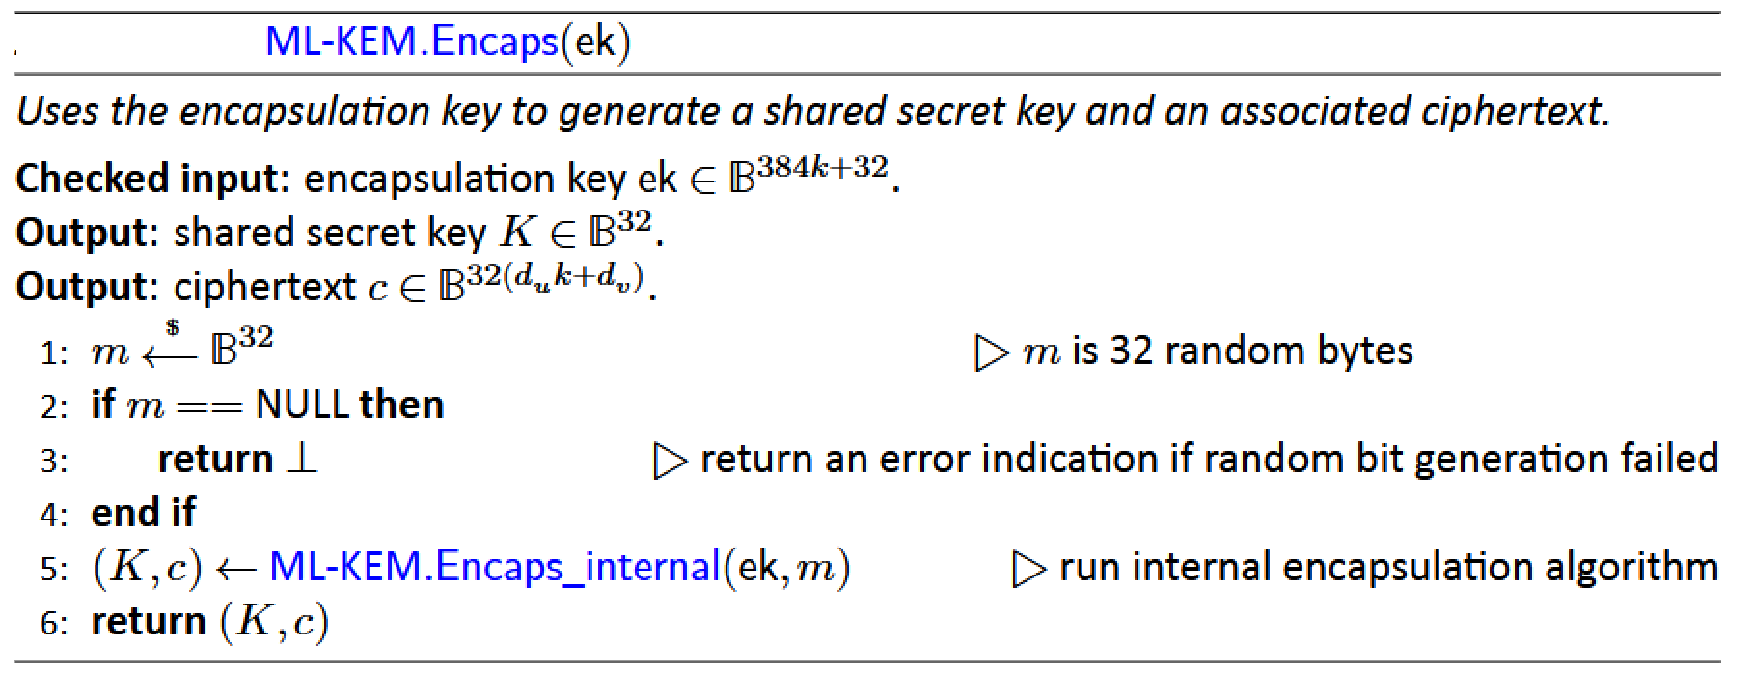
\includegraphics[width=.9\textwidth]{assets/pdfs/mlkem_encaps_edit.pdf}
	\captionsource
		{ML-KEM.Encaps() algorithm}
		{\cite{nistfips203}}
	\label{fig:mlkem-encaps}
\end{figure}

\begin{figure}[H]
	\centering
	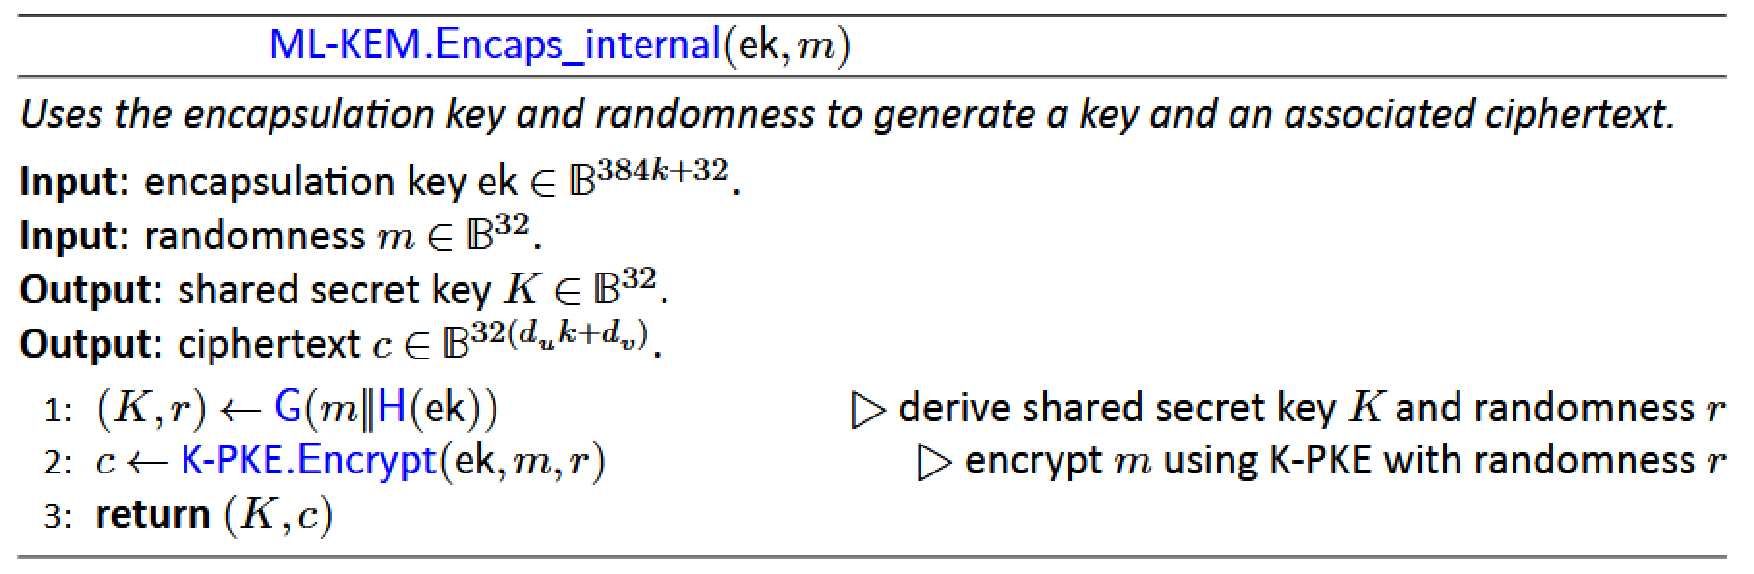
\includegraphics[width=.9\textwidth]{assets/pdfs/mlkem_encaps_internal_edit.pdf}
	\captionsource
		{ML-KEM.Encaps\_internal() algorithm}
		{\cite{nistfips203}}
	\label{fig:mlkem-encaps-internal}
\end{figure}

A copy of shared secret $K$ and the randomness $r$ used during encryption are obtained by hashing the encapsulation key and $m$. The randomness $r$, the encapsulation key, and $m$ are then used as input for Kyber’s encryption algorithm, K-PKE-Encrypt, which will encrypt $m$ into ciphertext.

\begin{figure}[H]
	\centering
	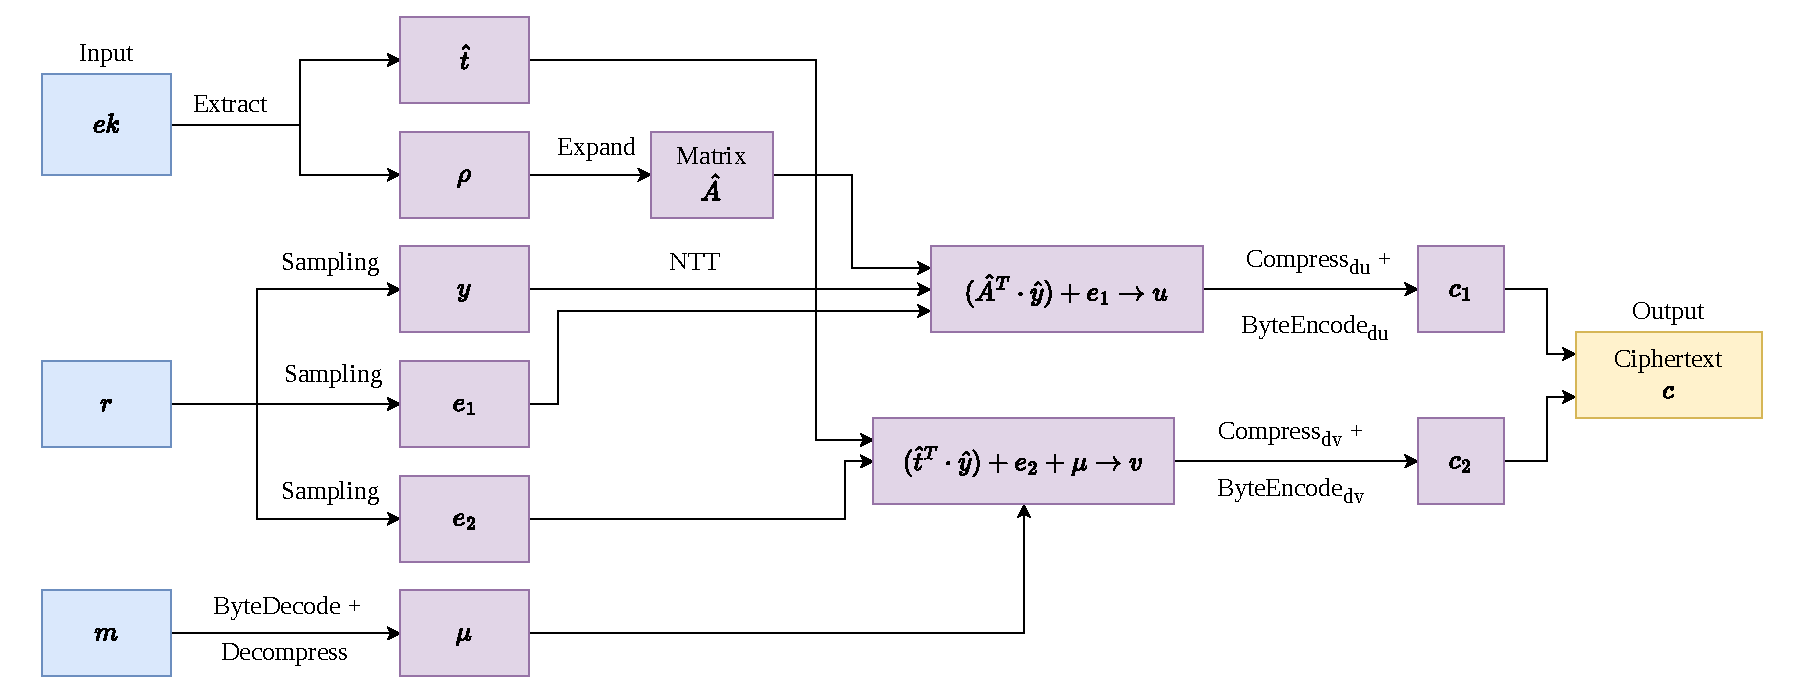
\includegraphics[width=1.0\linewidth]{assets/pdfs/kyber-encrypt.pdf}
	\caption{Kyber Encryption Algorithm K-PKE.Encrypt}
	\label{fig3}
\end{figure}

From the encapsulation key, $\hat{t}$ and seed $\rho$ are extracted. Matrix $\hat{A}$ is then re-expanded from $\rho$. If extracted correctly, both $\hat{t}$ and $\hat{A}$ should be the same as they were in K-PKE.KeyGen. 

Following that, the vector $y$ and noise terms $e_1$ and $e_2$ are sampled from centered binomial distribution using pseudorandomness from input randomness $r$. The ciphertext is then computed in two parts through the noisy equations $(\hat{A}^T \cdot \hat{y}) + e_1$ and $(\hat{t}^T \cdot \hat{y}) + e_2$. The encoding $\mu$ of message $m$ is added to the latter formula. The resulting pair $(u, v)$ is compressed and converted into a byte array before being output as the ciphertext.

\subsubsection{ML-KEM Decapsulation}
The decapsulation algorithm ML-KEM.Decaps accepts a decapsulation key and ciphertext generated by ML-KEM as input and outputs a shared secret key. This allows the recipient to recover the same secret value generated by the sender, enabling both parties to securely communicate using a common secret.

\begin{figure}[H]
	\centering
	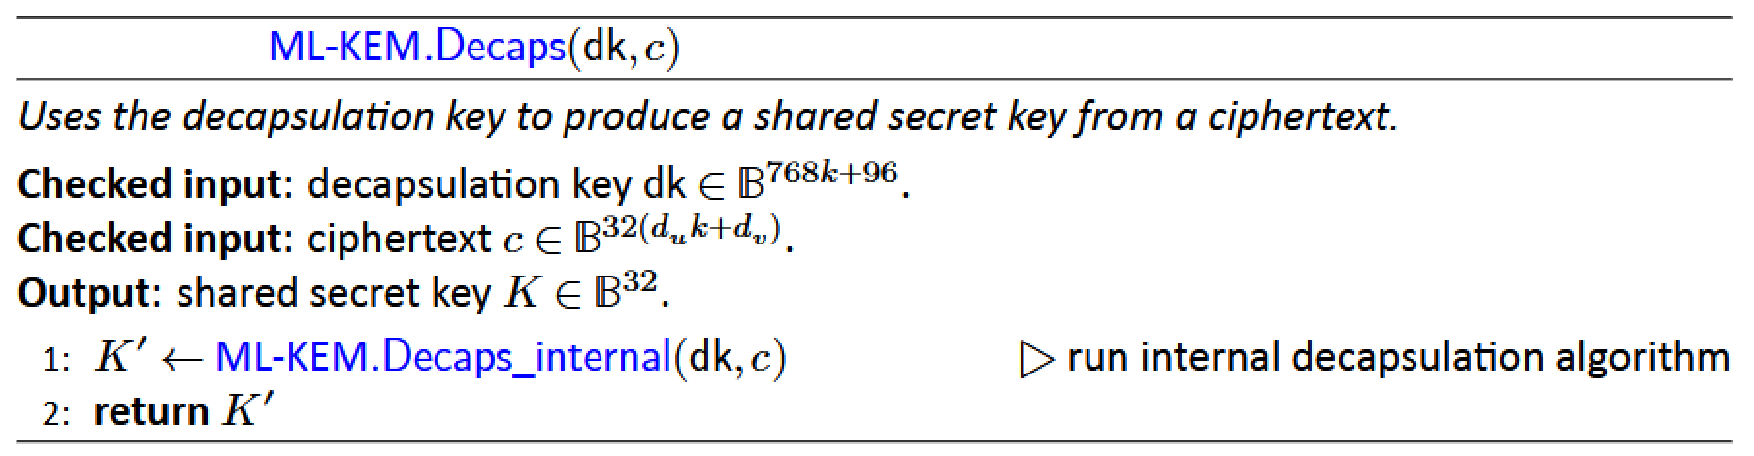
\includegraphics[width=.9\textwidth]{assets/pdfs/mlkem_decaps_edit.pdf}
	\captionsource
		{ML-KEM.Decaps() algorithm}
		{\cite{nistfips203}}
	\label{fig:mlkem-decaps}
\end{figure}

\begin{figure}[H]
	\centering
	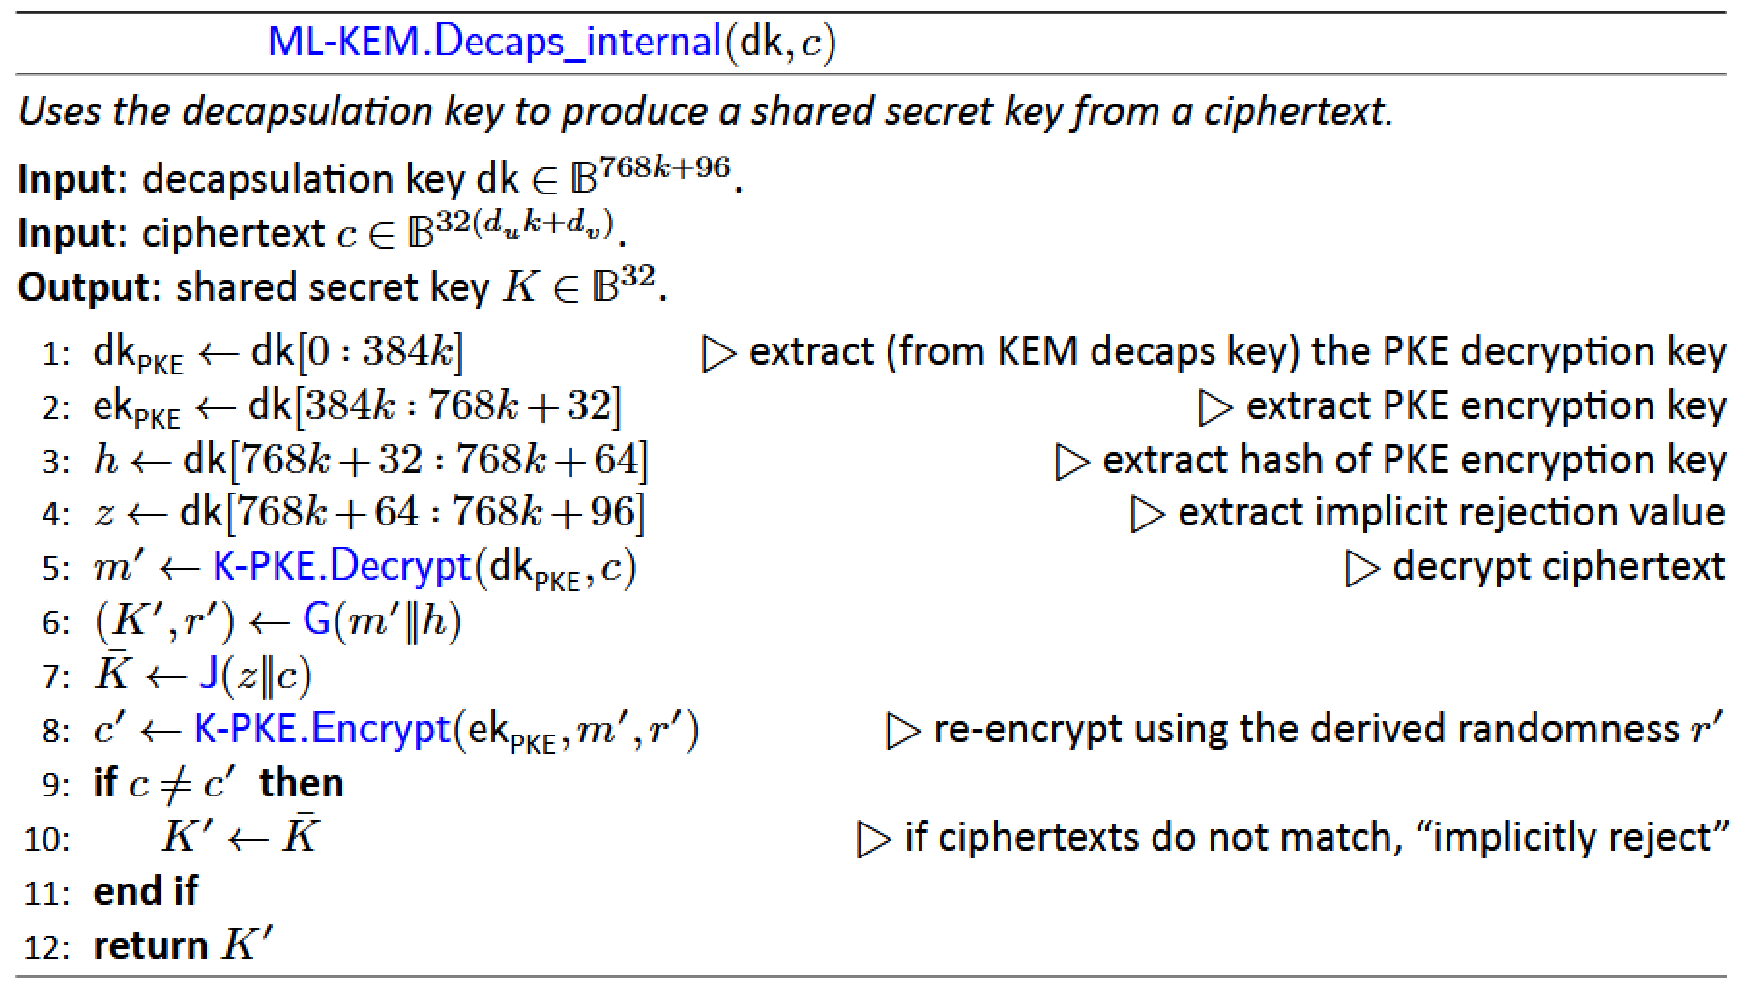
\includegraphics[width=.9\textwidth]{assets/pdfs/mlkem_decaps_internal_edit.pdf}
	\captionsource
		{ML-KEM.Decaps\_internal() algorithm}
		{\cite{nistfips203}}
	\label{fig:mlkem-decaps-internal}
\end{figure}

From the decapsulation key, the PKE encryption key $ek_{PKE}$, PKE decryption key $dk_{PKE}$, the hash value $h$ of the PKE encryption key, and random value $z$ are extracted. The ciphertext is decrypted through the K-PKE.Decrypt algorithm using the extracted decryption key, producing the plaintext message $m'$. The algorithm then re-encrypts the produced message into a new output ciphertext $c'$ along with computing candidate shared secret key $K'$ as done in the encapsulation stage. If the newly produced ciphertext does not match the input ciphertext, the algorithm performs an ’implicit rejection’, in which the value of $K'$ is replaced with a hash of $c$ appended to $z$. Otherwise, the decapsulation returns shared secret $K'$ unchanged.

\begin{figure}[H]
	\centering
	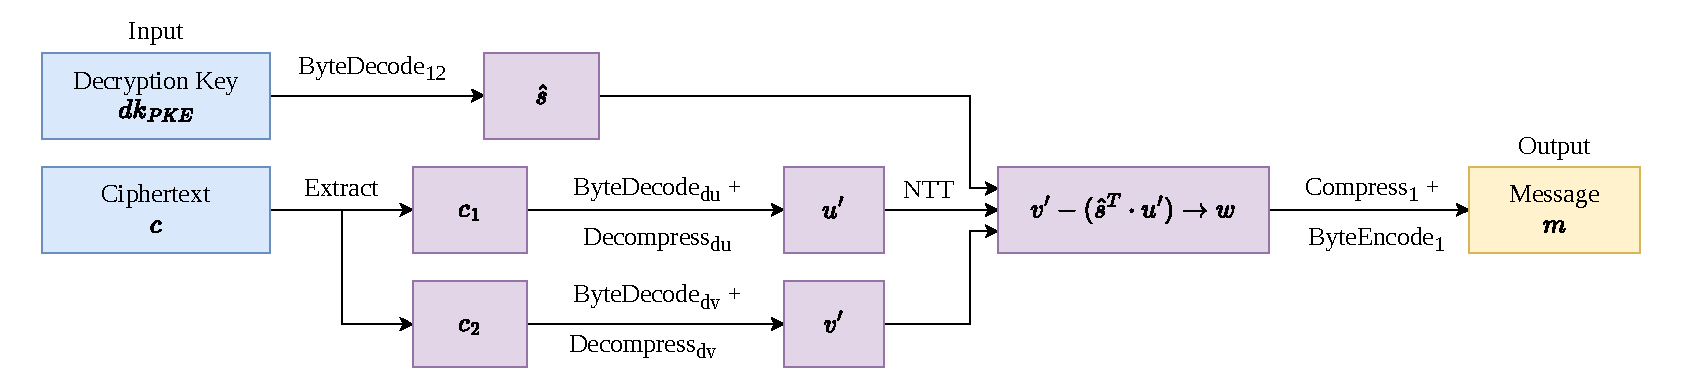
\includegraphics[width=1.0\linewidth]{assets/pdfs/kyber-decrypt.pdf}
	\caption{Kyber Decryption Algorithm K-PKE.Decrypt}
	\label{fig4}
\end{figure}

The K-PKE.Decrypt algorithm takes a decryption key and the corresponding ciphertext as inputs and extracts the secret variable $s$ and parts $c_1$ and $c_2$ from them respectively. Part $c_1$ is converted into $u'$ while $c_2$ is converted into $v'$. The true constant term $v$ is computed through $s^t \cdot u'$. The resulting $v$ is then subtracted from $v'$, outputting $w$, which is decoded into a plaintext message $m$.

\subsection{ML-DSA - FIPS 204}
ML-DSA, also known as Module-Lattice-Based Digital Signature Standard, is a standard set by NIST’s FIPS 204 publication that defines a method for digital signature generation and methods for the verification and validation of those signatures. The standard was proposed in response to the potential unreliability of modern digital signatures in the face of steady development of quantum computers.

ML-DSA is derived from the CRYSTALS-Dilithium algorithm \cite{2021dilithium}, whose security is based on the computational hardness of the MLWE and a nonstandard variant of MSIS (Module-Short Integer Solution) called SelfTargetMSIS. Both MLWE and MSIS (which relies on the hardness of SVP) are considered quantum resistant, and ML-DSA inherets that quality. 

ML-DSA and other digital signature schemes typically consist of three algorithms: a key generation algorithm, signing algorithm, and signature verifying algorithm.

\begin{figure}[H]
	\centering
	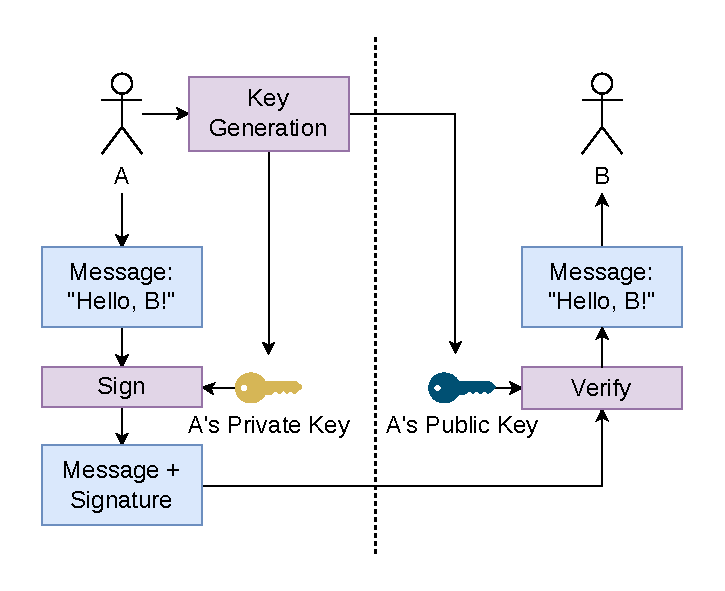
\includegraphics[width=.48\linewidth]{assets/pdfs/DSS_diagram.pdf}
	\caption{Simplified digital signature scheme}
	\label{fig5}
\end{figure}

As shown in Figure~\ref{fig5}, digital signature schemes are used to provide assurance that a digital message or document is authentic. Party A begins by running a key generation algorithm that produces a public and private key. The private key is kept by party A, while the public key is given to party B. When party A sends a message or document to party B, they run the signing algorithm using their private key and the message, which produces a signature. Party B then can, upon receiving it, verify the message’s authenticity using the corresponding public key.

ML-DSA also has three approved parameter sets. In order of least to most secure and most to least efficient, they are ML-DSA-44, ML-DSA-65, and ML-DSA-87.

\begin{figure}[H]
	\centering
	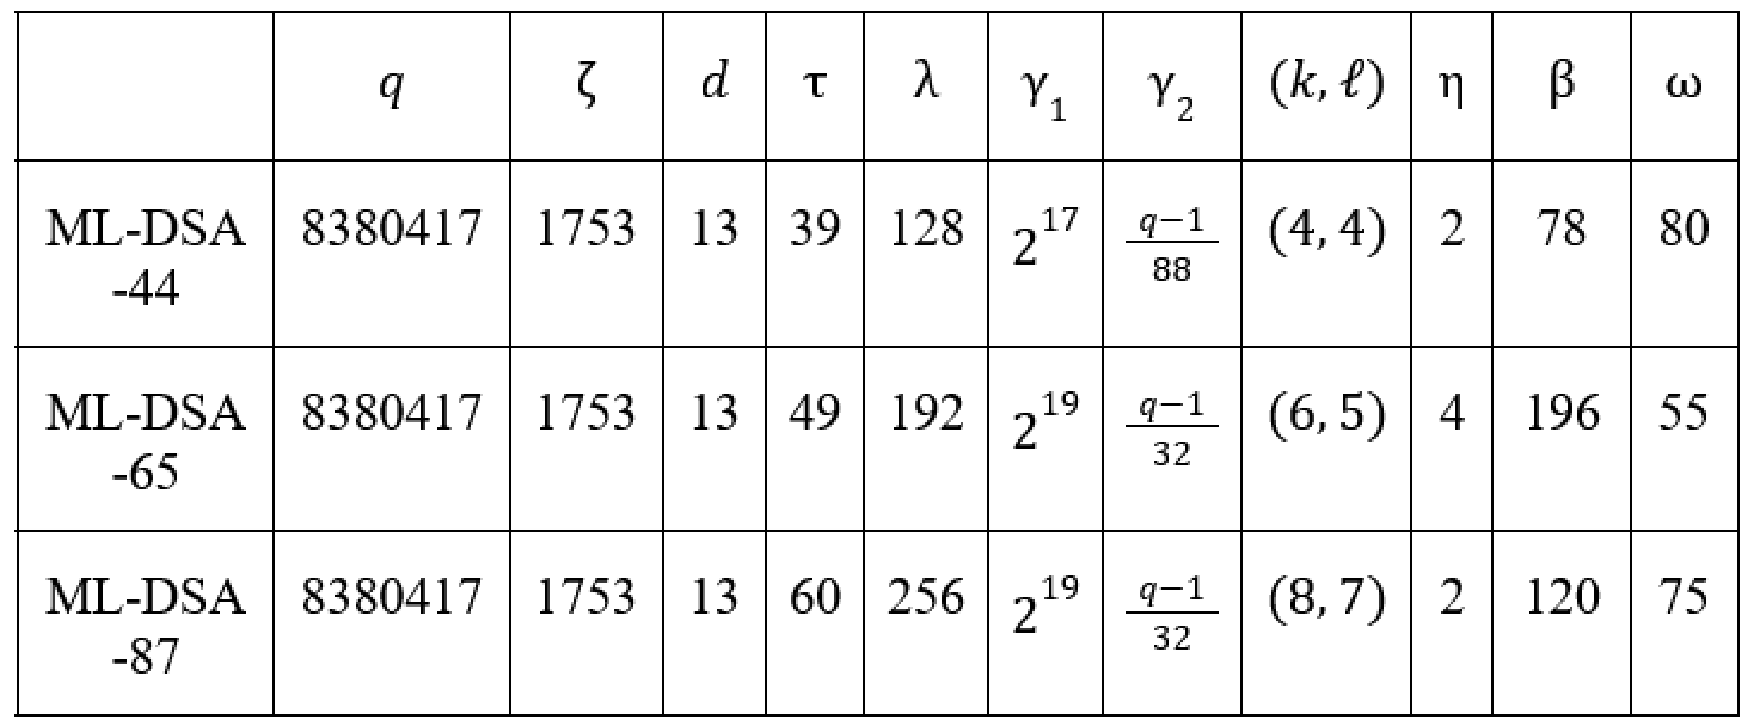
\includegraphics[width=.42\linewidth]{assets/pdfs/paramset_mldsa.pdf}
	\captionsource
        {Parameter sets for ML-DSA security levels}
        {National Institute of Standards and Technology (2024)}
	\label{fig:parameterdsa}
\end{figure}

Each parameter set is comprised of the variables $\tau$, $\lambda$, $\gamma_1$, $\gamma_2$, $(k, \ell)$, $\eta$, $\beta$, and $\omega$, along with the constants $q$, $\zeta$, and $d$.
\begin{itemize}
\item $\tau$ determines the number of $\pm1$'s in polynomial $c$ in the signing algorithm.
\item $\lambda$ determines the collision strength of $\tilde{c}$ by controlling the output length of the hash function that produces it.
\item $\gamma_1$ determines the coefficent range of polynomial vector $y$ in the signing algorithm. 
\item $\gamma_2$ determines the low-order rounding range used in the decomposition and hint-generation procedures during signing and verification.
\item $(k,\ell)$ determine the dimensions of matrix $A$ and the sizes of vectors used throughout the scheme. Larger values increase security at the cost of larger signatures and higher computational costs.
\item $\eta$ determines the coefficient range of the secret vectors $s_1$ and $s_2$. The coefficients are sampled from a small bounded distribution to ensure the resulting lattice vectors remain short.
\item $\beta$ defines the rejection bound used during signing. It limits the allowable size of coefficients in intermediate values to prevent leakage of secret information.
\item $\omega$ determines the maximum number of nonzero coefficients allowed in the hint vector $h$. This ensures that the hint remains sparse and compact.
\item $q$ is the modulus used for all polynomial coefficient arithmetic.
\item $\zeta$ is a primitive 512th root of unity in $\mathbb{Z}_q$ used in the Number Theoretic Transform (NTT).
\item $d$ determines the number of low-order bits discarded during the \texttt{Power2Round} decomposition procedure used in public key compression.
\end{itemize}
%Challenge entropy $\log_2 \binom{256}{\tau} + \tau$ & 192 & 225 & 257 \\
%\hline
%Repetitions & 4.25 & 5.1 & 3.85 \\
%\hline
%Claimed security strength & Category 2 & Category 3 & Category 5 \\
%\hline

\subsubsection{ML-DSA Key Generation}
ML-DSA.KeyGen generates a public key and a private key from a randomly selected 32-byte seed $\xi$. The public key allows for others to verify signatures, while the private key is used to create them and has to remain secret. The seed itself is generated using an approved RBG (Random Bit Generator) such as those described by Barker et al \cite{barker2015sp80090a,barker2018sp80090b,barker2025sp80090c}.

\begin{figure}[H]
	\centering
	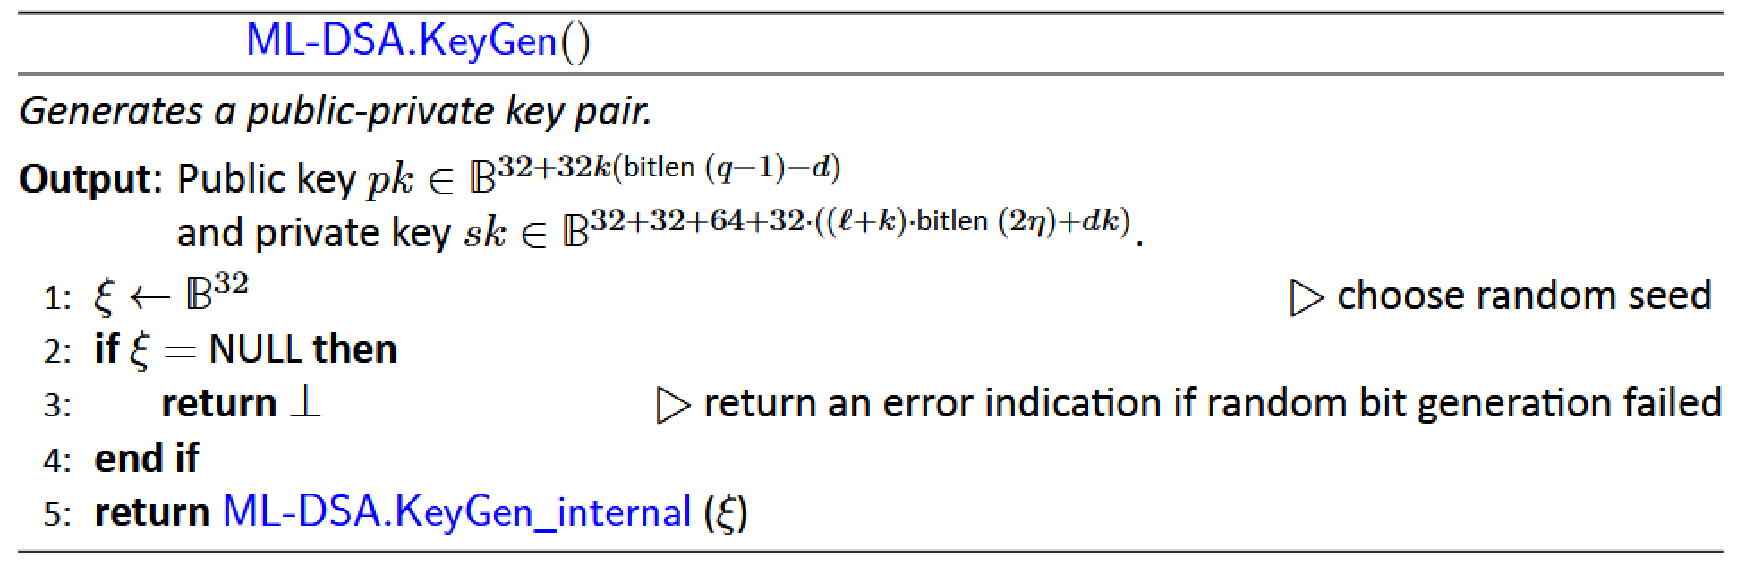
\includegraphics[width=.9\textwidth]{assets/pdfs/mldsa_keygen_edit.pdf}
	\captionsource
		{ML-DSA.KeyGen() algorithm}
		{\cite{nistfips204}}
	\label{fig:mldsa-keygen}
\end{figure}

\begin{figure}[H]
	\centering
	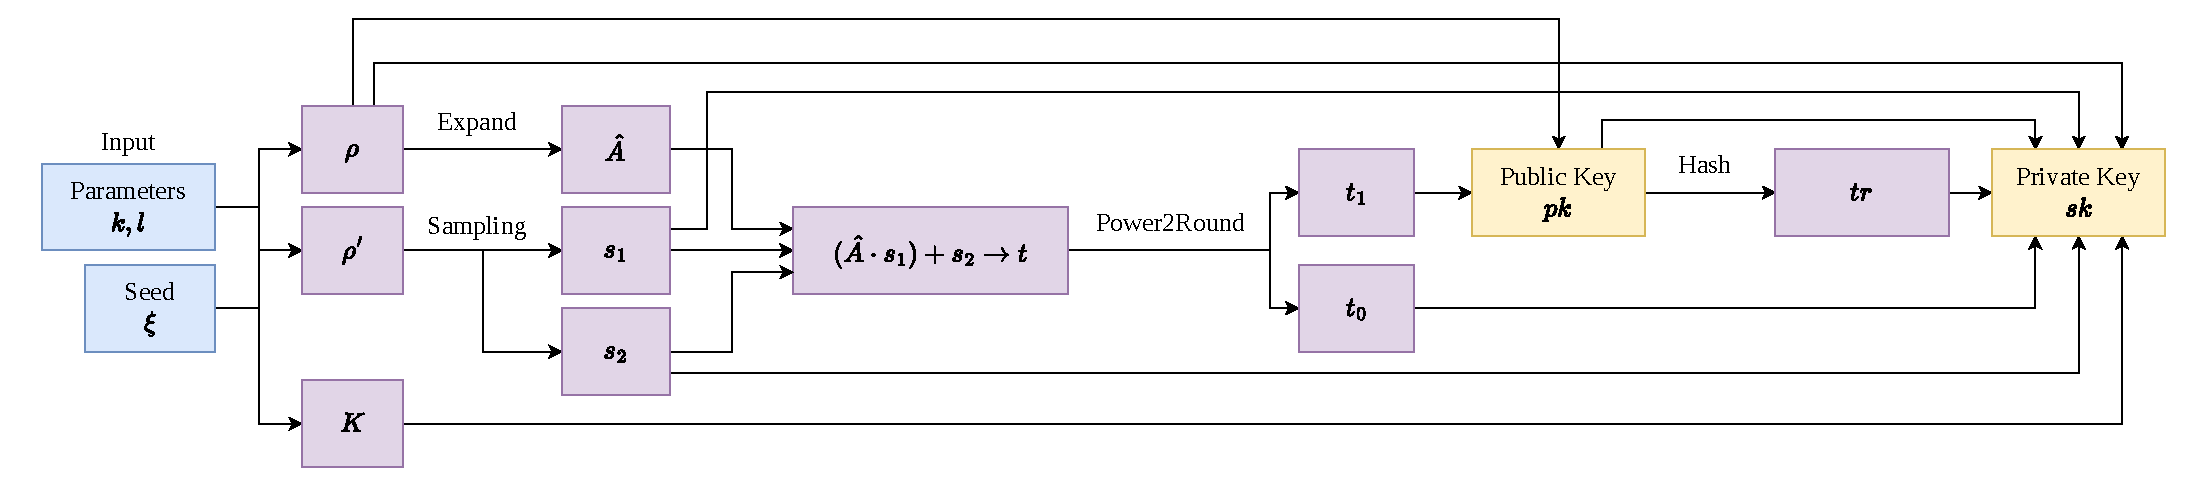
\includegraphics[width=1.0\linewidth]{assets/pdfs/dsa-keygen.pdf}
	\caption{ML-DSA Internal Keygen Algorithm ML-DSA.KeyGen\_internal}
	\label{fig6}
\end{figure}

The seed $\xi$ is expanded into 32 byte random seed $\rho$, 64 byte random seed $\rho'$, and 32 byte random seed $K$. Seed $\rho$ is expanded into matrix $A$ through sampling, and secret polynomial vectors $s_1$ and $s_2$ are sampled using seed $\rho'$. The three together compute part $t$ of the public key, of which is decomposed into its higher and lower order components, $t_1$ and $t_0$ for the purposes of compression. The generated public key is formed by encoding the seed $\rho$ together with $t_1$. The private key is composed of encoded representations of the seed $\rho$, the signing seed $K$, the hash of the public key $tr$, the secret vectors $s_1$ and $s_2$, and $t_0$.

\subsubsection{ML-DSA Signing}
The signing algorithm ML-DSA.Sign takes a private key, a formatted message, and a context string (a byte string of 255 or fewer bytes) as input and generates a signature encoded as a byte string. The resulting signature can be used to confirm both the origin of the message and that its contents have not been modified after signing.

\begin{figure}[H]
	\centering
	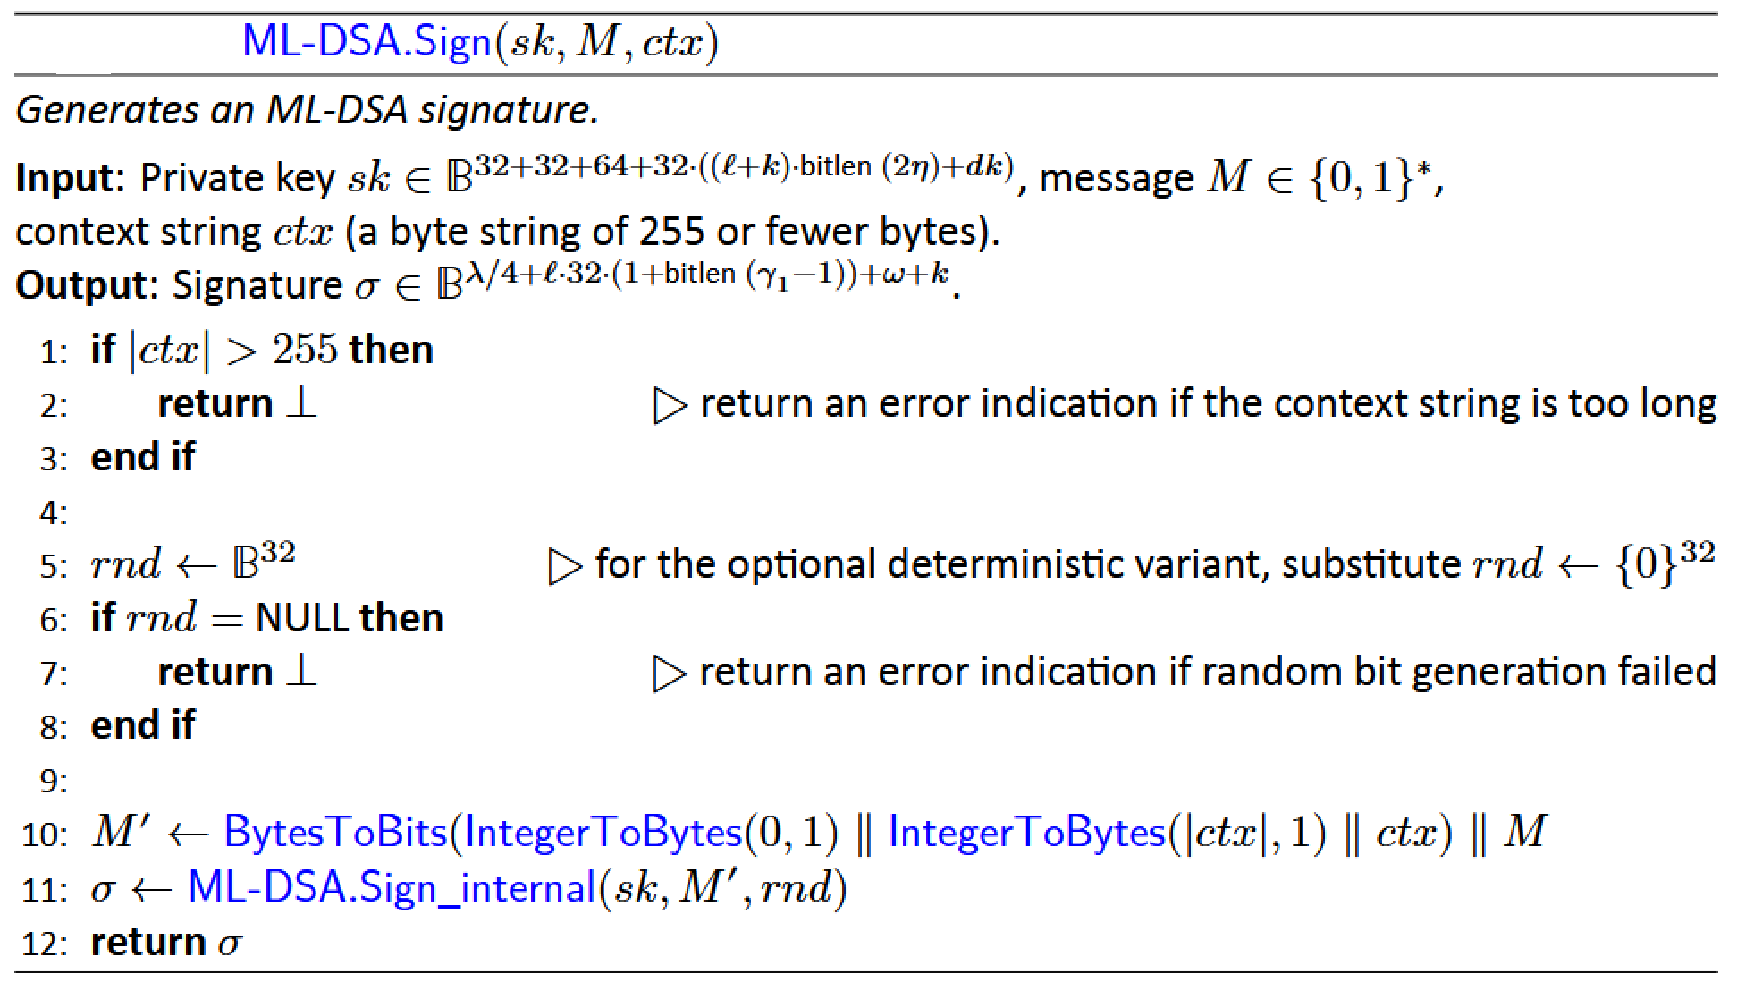
\includegraphics[width=.9\textwidth]{assets/pdfs/mldsa_sign_edit.pdf}
	\captionsource
		{ML-DSA.Sign() algorithm}
		{\cite{nistfips204}}
	\label{fig:mldsa-sign}
\end{figure}

\begin{figure}[H]
	\centering
	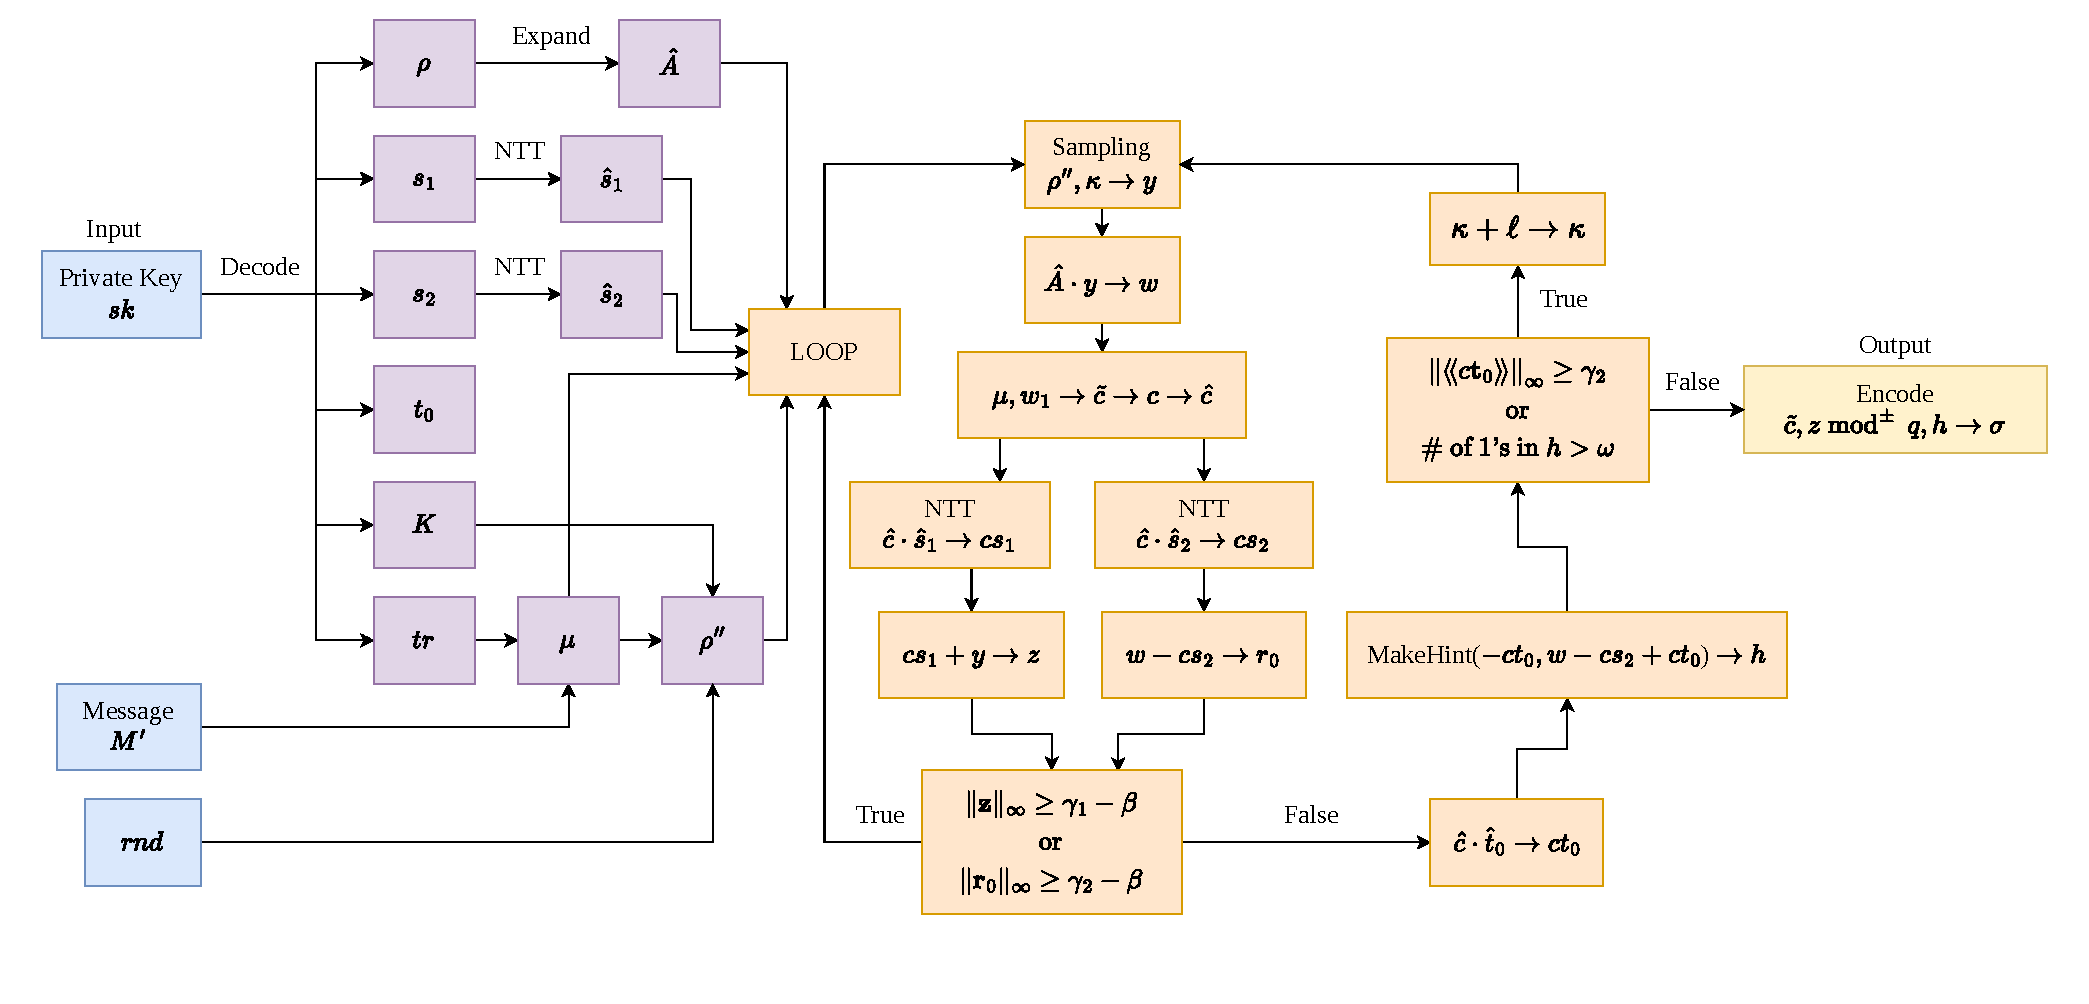
\includegraphics[width=1.0\linewidth]{assets/pdfs/dsa-sign.pdf}
	\caption{ML-DSA Internal Signing Algorithm ML-DSA.Sign\_internal}
	\label{fig7}
\end{figure}

From the private key, the signer extracts the following: public random seed $\rho$, private random seed $K$, the hash of the public key $tr$, secret polynomial vectors $s_1$ and $s_2$, and lower order component of part $t$ of the public key $t_0$. Seed $\rho$ is then reexpanded into matrix $A$ as in the key generation algorithm. Message $M$ is concatenated to $tr$ and hashed into 64 byte message representative $\mu$. A 64 byte seed $\rho''$ is then produced for private randomness during each signing operation by hashing into 64 bytes a concatenation of $K$, random 32 byte string value $rnd$, and $\mu$.

Following that, a rejection sampling loop that produces a signature is repeated until a valid one is created, which is then encoded as a byte string and output. The main computations involved in the loop are as follows:
\begin{itemize}
	\item Generate vector $y$ from using the ExpandMask function with $\rho$ and counter $\kappa$ as inputs. 
	\item Commitment $w_1$ is computed by taking the higher order component of $w$, computed through $A \cdot y$.
	\item $w_1$ and $\mu$ are concatenated and hashed to produce the commitment hash $\tilde{c}$. $\tilde{c}$ is then used to pseudorandomly sample a polynomial $c$ that has coefficients \( \lbrace -1, 0, 1 \rbrace \) and Hamming weight $\tau$.
	\item Response $z = y + cs_1$ is computed. $r_0$ is also computed by taking the lower order components of $w - cs_2$. Both are used in validity checks that, if failed, restart the loop.
	\item If the validity checks pass, hint polynomial $h$ is computed using the MakeHint function, which will allow the later verifier to reconstruct $w_1$ and other components of the signature correctly. After running more checks to see whether the coefficients in $ct_0$ are within a certain boundary and that the number of 1's in $h$ does not exceed $\omega$, assuming both checks pass, the final signature consisting of a byte encoding of commitment hash $\tilde{c}$, the response $z$, and the hint $h$ will be output.
\end{itemize}

\subsubsection{ML-DSA Verification}
The verification algorithm ML-DSA.Verify accepts a public key, a message, a signature, and a context string as input and returns a boolean value indicating whether the signature is valid. If it is true, the signature corresponds to the given message and public key. If it is false, the signature is invalid. As a result, anyone possessing the public key can verify if a message originated from the holder of the corresponding private key and has not been modified since it was signed. 

\begin{figure}[H]
\centering
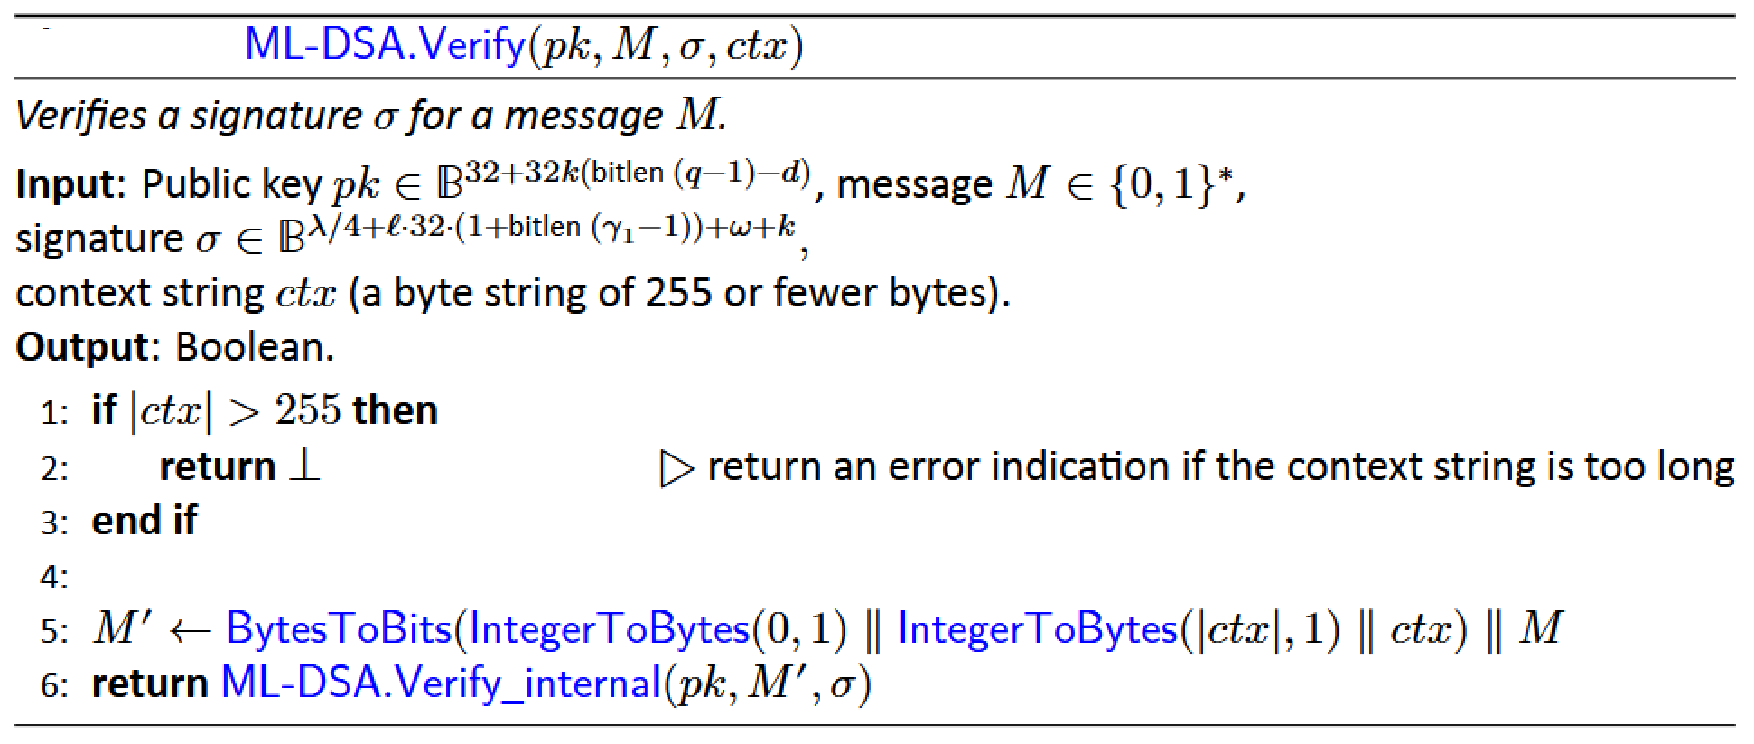
\includegraphics[width=.9\textwidth]{assets/pdfs/mldsa_verify_edit.pdf}
\captionsource
	{ML-DSA.Verify() algorithm}
	{\cite{nistfips204}}
\label{fig:mldsa-verify}
\end{figure}

The verifier starts by extracting public random seed $\rho$ and vector $t_1$ from the public key, then the commitment hash $\tilde{c}$, response $z$, and hint $h$ from the signature. $h$ is checked to see if it was encoded properly; if not, then the algorithm returns false. Otherwise, matrix $A$ is expanded from $\rho$, $tr$ is hashed from the public key and concatenated with the message input $M'$, then hashed again to create message representation $\mu$. The verifier's challenge $c$ is computed from $\tilde{c}$ as in the signing algorithm.

The verifier then attempts to reconstruct the signer's commitment $w_1'$. In the verifier algorithm, $w_1'$ requires $w'_{approx}$, which is computed through $A \cdot z - c \cdot (t_1 \cdot 2^d)$. $w_1$ is reconstructed by running the algorithm UseHint, which takes $w'_{approx}$ and recovers the high bits of the $w_1$ calculated during signing using $h$. The result is concatenated to $\mu$ and hashed to create $\tilde{c}'$.

Finally, the verifier checks that response $z$ is valid (by checking whether all coefficients in $z$ are smaller than bound $\gamma_1 - \beta$) and that $\tilde{c}$ matches with $\tilde{c}'$. If both checks succeed, the verifier returns true. Otherwise, it returns false.

\begin{figure}[H]
	\centering
	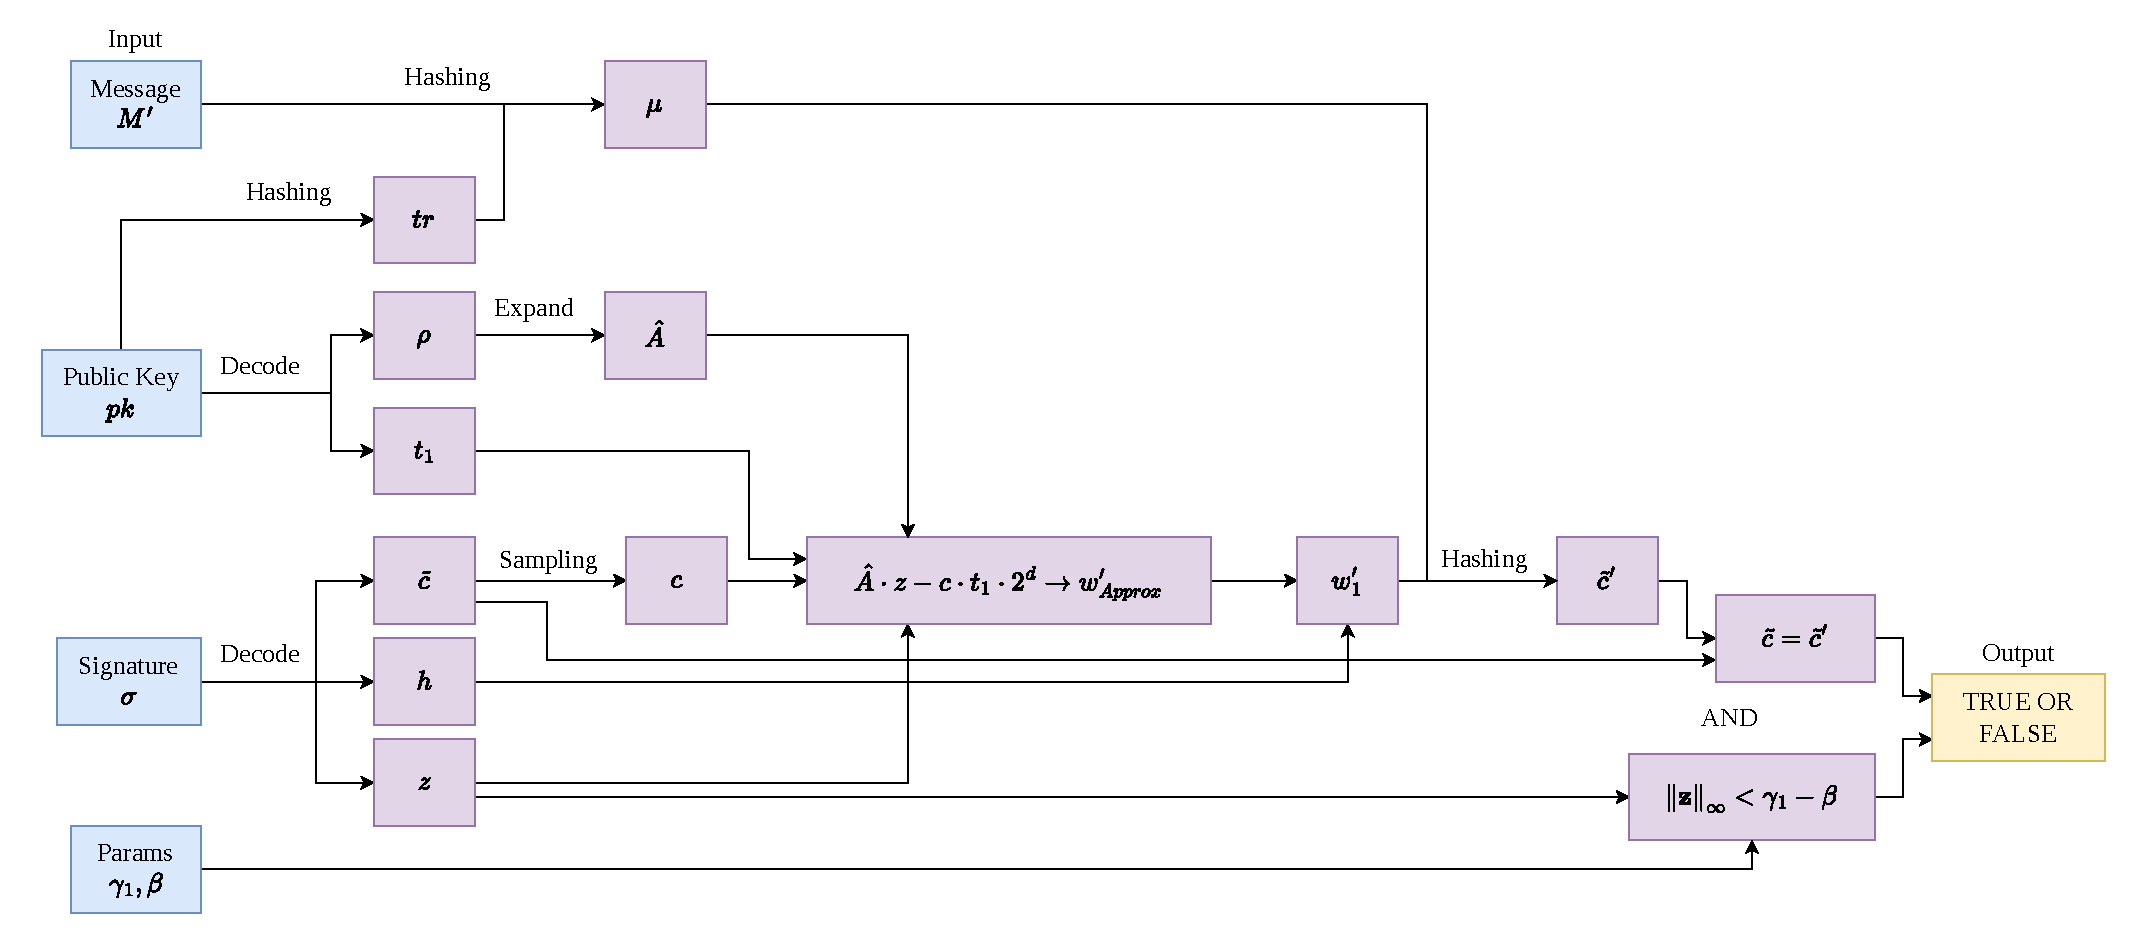
\includegraphics[width=1.0\linewidth]{assets/pdfs/dsa-verify.pdf}
	\caption{ML-DSA Internal Verification Algorithm ML-DSA.Verify\_internal}
	\label{fig8}
\end{figure}

\subsection{LLL}
The LLL (Lenstra-Lenstra-Lovasz) cryptanalysis algorithm is a lattice reduction algorithm developed by Arjen Lenstra, Hendrik Lenstra, and Laszlo Lovasz in 1982. Although LLL is now largely ineffective for reducing lattices in many PQC algorithms such as ML-KEM and ML-DSA, the it is the foundation of modern lattice reduction cryptanalysis. For example, it serves as the foundation of BKZ, the upscaled version of LLL, by having several LLL processes executed for a single BKZ process. 

\begin{figure}[htbp]
    \centering
    
\includegraphics[width=0.7\textwidth]{assets/pdf/LLLRev.pdf}
    \caption{The LLL algorithm}
    \label{LLL}
\end{figure}
\mbox{}

In the Figure~\ref{LLL}, we can see how the algorithm works. The inputs are in the form of matrices, or a set linear equations. For a single LLL process, the input is in the form of a lattice basis $L$, which is in the form of a set of basis vectors ${\{v_1, v_2, ....v_n\}}$. Every vector within the set will be iteratively processed by Gram-Schmidt orthogonalization, then reduction or swap, and then examined whether the basis at the index fulfills the Lovasz Condition or not. The iteration process, however, is controlled by a pointer variable $k$ which starts from 2nd index to the $n$-th index (the last vector). In other words, the first vector only acts as a projection reference for Gram-Schmidt orthogonalization (it only acts as the initial orthogonal basis ($\mathbf{v}_1^* = \mathbf{v}_1$)) and size reduction processes of subsequent vectors, but the first vector is never individually subjected to the vector swap mechanism (unless during the first iteration, the second vector fails to meet the Lovász Condition checking) or Lovász Condition checking. After all subsequent vectors have gone through these processes, the loop ends and the algorithm stops. 

Unless the initial lattice basis is already a highly orthogonal basis, we will obtain a more orthogonalized and shorter version of the basis. Thus, with a basis that is more orthogonal and shorter, we would have it easier for recovering the LWE small errors hidden in the linear equations that form the public matrix we want to crack. 

As an important note, the $\delta$ value used in Lovász Condition ranges from 0.25 as the minimum value to 0.99 as the maximum value. A higher $\delta$ yields higher quality outputs at the expense of more iterations, and a lower $\delta$ leads to fewer iterations at the expense of lower quality outputs. In other words, a higher $\delta$ makes the recovery of the LWE errors easier.

Below is the explanation of the LLL steps : 
\begin{enumerate}
    \item \textbf{Initialization.} $$\mathbf{L} = \{v_1, v_2, ....v_n\}$$ $L$ is a lattice basis to be reduced, with $n$ vectors within it. $L$ contains ${\{v_1, v_2, ....v_n\}}$. Assume $L$ is a "bad" basis, then the goal is to make it more orthogonal and shorter. 
    \item \textbf{Gram-Schmidt orthogonalization.}. $$\mathbf{v}_k^* = \mathbf{v}_k - \sum_{j=1}^{k-1} \frac{\langle \mathbf{v}_k, \mathbf{v}_j^* \rangle}{\|\mathbf{v}_j^*\|^2} \mathbf{v}_j^*$$
    Right after the initialization, the algorithm processes the basis vectors sequentially. At the global scale (or the outer loop) in $L$, the algorithm performs Gram-Schmidt orthogonalization (GSO) for all vectors in $L$, then produces the initial orthogonalized $\mathbf{v}_k^*$ and their corresponding projection coefficients $\mu_{k,j}$, with $1 \le j < k \le n$ before the main loop execution begins. Notice that for the first vector ($k = 1$), no projection is needed since it has no preceding vectors. Hence, $\mathbf{v}_1^* = \mathbf{v}_1$.
    \item \textbf{Main loop.} After the global Gram-Schmidt orthogonalization process, the index pointer $k$ points at the second vector from the left (the vector of $v_2$), thus the main loop begins with the first iteration at $k=2$.
    \item \textbf{Basis reduction loop.} The algorithm checks the size of the vector, and then performs a size reduction of the vector to ensure that the length of the projection coefficients satisfies: $$|\mu_{k,j}| \leq 0.5$$. To satisfy the condition, the algorithm uses an internal index pointer, $j$, whose sole purpose is to become the backward iterator in this basis reduction loop. This loop starts from $j = k - 1$ and continues until $1$. This ensures that the current target vector $\mathbf{v}_k$ is systematically reduced against all of its preceding vectors in the basis. The vector $\mathbf{v}_k$ is then iteratively updated using the following formula : $$\mathbf{v}_k \leftarrow \mathbf{v}_k - \lfloor\mu_{k,j}\rceil\mathbf{v}_j$$. Concurrently, to maintain mathematical consistency with the modified vector components, the algorithm must update $\mathbf{v}_k^*$ and the corresponding projection coefficients $\mu_{k,j}$ by fully recomputing the entire Gram-Schmidt orthogonalization sequence to get the updated $\mathbf{v}_k^*$ and $\mu_{k,j}$ values whenever $\mathbf{v}_k$ is modified inside this basis reduction loop. The basis reduction loop continues until the backward iterator $j$ has fully decreased past $1$, signifying that the $\mathbf{v}_k$ has been checked and reduced against every preceding vector in the basis $L$. Once the basis reduction loop ends, the updated vector is then subjected to the core step of the LLL algorithm - the Lovász Condition checking.
    \item \textbf{Lovasz Condition checking.} $$\|\mathbf{v}_k^*\|^2 \ge \left(\delta - \mu_{k,k-1}^2\right)\|\mathbf{v}_{k-1}^*\|^2$$ Using the updated $\mathbf{v}_k^*$ obtained from the preceding basis reduction loop, the algorithm evaluates whether the current vector ordering satisfies the Lovász Condition or not. Should the basis at the current iteration satisfies the Lovasz Condition, it will proceed to check whether all vectors have been examined. If that's the case ($k >= n$), then the main loop terminates, signifying that the entire basis has been successfully reduced, and followed immediately by the termination of the algorithm altogether. If not, then the iteration continues and $k$ will point to the next vector ($k \leftarrow k + 1$), continuing the main loop until all vectors in the basis $L$ have been fully processed. However, if the basis fails to satisfy the Lovasz Condition at the current iteration, a vector swap mechanism is executed and followed by a re-evaluation of the basis sequence.
    \item \textbf{Vector swap.} If the current basis configuration does not satisfy the Lovász Condition at index $k$, it implies that the vector $\mathbf{v}_k$ has a significantly shorter orthogonal projection compared to its predecessor, $\mathbf{v}_{k-1}$, which makes the ordering of the vectors within $L$ deficient. To fix this ordering deficiency, a vector swap mechanism must be executed. The order of the two adjacent vectors within the basis is interchanged as follows:
    \begin{equation}
    \mathbf{v}_{k-1} \leftrightarrow \mathbf{v}_k
    \end{equation}
    Since this swap alters the geometric orientation and structural sequence of $L$, the previously calculated Gram-Schmidt vectors and coefficients become invalid from index $k-1$ onwards. Consequently, the algorithm retreats its main loop iteration counter using the following step :
    \begin{equation}
    k \leftarrow \max(k-1, 2)
    \end{equation}
    This repositioning ensures that the counter shifts backward by one step, forcing the algorithm to recompute the local Gram-Schmidt orthogonalization and re-apply the basis reduction at this lower index before the Lovász Condition can be re-evaluated. As the important note, the $\max$ function serves as a logical guardrail to prevent $k$ from accessing indices lower than $2$.
    \item \textbf{Output}. After all of the vectors have been examined and $L$ meets the Lovasz Condition requirement, the algorithm terminates and returns a more orthogonalized and shortened version of $L$. This reduced lattice basis is more useful for recovering hidden LWE errors embedded within the linear equations. 
    
\end{enumerate}

\subsection{BKZ}
\begin{figure}[htbp]
    \centering
    
\includegraphics[width=0.7\textwidth]{assets/pdf/BKZRev.pdf}
    \caption{The BKZ algorithm}
    \label{BKZ}
\end{figure}
\mbox{}
The BKZ (Block Korkine-Zolotarev) lattice reduction algorithm was first proposed by Clauss-Peter Schnorr in 1987, and in 1994 he and Martin Euchner published the journal of the BKZ algorithm \cite{13}. This lattice reduction algorithm, while based on LLL, is much more stronger compared to LLL. Nowadays, the usage of BKZ in cryptanalysis is common, as the algorithm becoming increasingly important due to the emergence of the lattice-based post-quantum cryptographic algorithms \cite{14}. 

Like in the LLL algorithm, the goal is to make $L$ more orthogonal and shorter. The steps of the BKZ algorithm are explained below : 

\begin{enumerate}
    \item \textbf{Initialization and the first LLL.} The first step in BKZ algorithm is to run an LLL process, symbolized with $$\mathbf{LLL(L, \delta)}$$ on $n$ vectors within ${\{v_1, v_2, ....v_n\}}$. As a side note, the $\delta$-value used in BKZ for all LLL executions within a BKZ algorithm execution is the same, and normally the $\delta$ value used is 0.99. This is done to ensure a more orthogonalized and shorter outputs for each LLL execution and the final output of the BKZ execution as well.
    \item \textbf{Main iteration.} After the first global LLL process has been completed, the algorithm begins the main iteration. While the LLL process iteratively processes the vectors one-by-one across the entire basis (for a single iteration in LLL, only one vector is reduced), BKZ processes vectors within localized regions of the basis called blocks. Think of it as a pointer that points $\beta$ neighbouring vectors for each iteration, and performs SVP searching, vector swapping, and localized LLL, all exclusively for all vectors that are currently pointed. After the localized LLL is done, the pointer shifts just one vector to the right. So in other words, the block structure in BKZ behaves more like a sliding window with a fixed block size $\beta$ that traverses the lattice basis from left to the right, and performs SVP enumeration, vector swapping, and LLL only for all vectors within the block. For each single iteration, the BKZ algorithm selects a local block from the basis:$$\mathbf{L}_{[i,h]} = \{v_i, v_{i+1}, ....v_h\}$$ in which $$\mathbf{h} = \mathbf{max}(i+\beta-1, n)$$. Here, $i$ is the starting index and $h$ last index of the current block, while $\beta$ is the fixed block size of the entire BKZ algorithm. For example, we have $\mathbf{L} = \{v_1, v_2, v_3, v_4, v_5\}$ with $\beta = 3$. The first block would be $\mathbf{L}_{[1,3]} = \{v_1, v_2, v_3\}$ and after the first iteration ends, the next iteration's block would be $\mathbf{L}_{[2,4]} = \{v_2, v_3, v_4\}$. As we see,the "sliding window" only moves by one vector to the left, which is why the BKZ's blocks are overlapping to each other. As an important note, since $\beta$-value is the symbolization of the block size, it means that the $\beta$-value determines how many neighboring vectors are included inside the current block during each iteration, and as such, the selection of the $\beta$-value has a big role on determining the quality of the BKZ's output. A smaller $\beta$ produces smaller blocks, which means it produces a faster execution of the algorithm with the cost of the BKZ's output, while a bigger $\beta$ resulted in slower execution but with better output.
    \item \textbf{Localized SVP enumeration and LLL.} After the block formation, the BKZ algorithm searches the shortest non-zero vector (SVP) inside the current block. Shall the SVP candidate $v$ is deemed to be shorter enough compared to the currently examined basis vector (as mathematically stated below) : $$||v|| < \beta||b_i||$$, then the SVP candidate $v$ is deemed to be an improvement to the basis structure. Thus, the candidate v is inserted into the basis at the current block position $(v,b_i,b_{i+1}...,b_h)$. Also usually known as nontrivial insertion. Should the condition $||v|| \ge \beta||b_i||$ happens, then no insertion would be done, since the algorithm doesn't consider this case as an impactful improvement of the basis quality. After the local SVP enumeration, a localized LLL process is executed, which only involves all vectors within the current block. 
    \item \textbf{Termination and the resulted output.} Once all blocks within the lattice basis have been examined and processed, and no further nontrivial insertion can be executed, the BKZ algorithm terminates. Like the LLL algorithm, it would produce a shorter and more orthogonalized lattice basis compared to the initial basis.
\end{enumerate}

Because the BKZ algorithm is formed from a global LLL, followed by the execution of localized LLL reductions and localized SVP enumerations in each of its blocks, the quality of a BKZ output is generally better (the output is expected to be much shorter and much more orthogonalized) than the output produced from a single LLL process. Thus, recovering LWE errors hidden in the system of linear equations within a lattice-based post-quantum cryptographic system is generally better be done with BKZ. The only downside from a BKZ execution compared with LLL is the computational cost, since a single BKZ process involves several LLL processes. 